\documentclass[conference]{IEEEtran}
\IEEEoverridecommandlockouts

\usepackage{cite}
\usepackage{amsmath,amssymb,amsfonts}
\usepackage{graphicx}
\usepackage{booktabs}
\usepackage{multirow}
\usepackage{xcolor}
\usepackage{url}

\graphicspath{{figures/}}

% 修复实验相关内容集中在 remedy.tex，结果出来后只改那一个文件
% 修复实验的内容集中在这里，等 run_remedy.sh 的结果出来后只改这一个文件。

\newcommand{\REMEDYABSTRACT}{%
Both mechanisms are real, and one of them is locally actionable: reweighting the
objective towards the decision region raises enhancing-tumour Dice from $0.228$
to $0.306$, a gain that is significant in ten of twelve patient-paired cells,
but it costs $0.222$ whole-tumour Dice, and reweighting towards the amplified
late-time region degrades every region. Neither recovers the method. The
failure therefore lies in the conditioning of the regression target rather than
in the allocation of the loss.%
}

\newcommand{\REMEDYINTRO}{%
Finally we ask whether the two mechanisms are \emph{actionable}. If the collapse
were caused by the loss misallocating capacity, then correcting the allocation
should help. Section~\ref{sec:remedy-results} reweights the same objective along
the two axes the diagnostic identified and reports both what improves and what
does not.%
}

\newcommand{\REMEDYCONTRIB}{%
A test of two loss reweightings derived from those mechanisms, showing that the
decision-region mechanism is locally actionable --- it closes a fifth of the
enhancing-tumour gap to the discriminative model --- while neither reweighting
rescues whole-tumour segmentation. This locates the failure in the
parameterisation of the regression target rather than in the allocation of the
loss.%
}

\newcommand{\REMEDYSECTION}{%
\subsection{Are the diagnosed mechanisms actionable?}
\label{sec:remedy-results}

Table~\ref{tab:remedy} reports the two reweightings and their combination, each
trained at three seeds with everything else identical to the baseline. Neither
recovers whole-tumour segmentation, and the two axes behave very differently.

\paragraph{Foreground weighting is locally effective but costs the primary
metric.}
Raising the weight of non-background voxels by $10\times$ --- the direct
response to the observation that background occupies over $80\%$ of the sampled
volume at two orders of magnitude lower error --- raises enhancing-tumour Dice from
$0.228$ to $0.306$, a relative gain of $34\%$, and leaves tumour-core Dice
essentially unchanged ($0.372$ against $0.360$). Patient-paired bootstrap gives
a positive interval in ten of the twelve (seed, missing-pattern) cells for ET,
against only one negative. The mechanism is therefore real: the background did
dominate the objective, and the smallest class was the one paying for it.

But whole-tumour Dice falls from $0.553$ to $0.331$, with eleven of twelve cells
significantly negative and a mean paired difference of $-0.222$. The remedy
trades the primary metric for the rarest one; it does not rescue the method.
That the two regions move in opposite directions is itself informative: the
velocity field is a single global object, so re-weighting voxels does not
reallocate capacity within the field, it changes the field the model converges
to. The background-dominated objective was evidently not the binding constraint
on whole-tumour accuracy.

\paragraph{Weighting the amplified region makes everything worse.}
If the $1/(1-t)$ amplification of Eq.~\eqref{eq:sensitivity} were the operative problem, putting
capacity where the amplification acts should help. It does the opposite: the
late-time weight lowers whole-tumour Dice to $0.393$ (nine of twelve cells
significantly negative), tumour-core to $0.237$ (ten of twelve) and
enhancing-tumour to $0.110$ (nine of twelve). Combining both factors is worse
still on whole-tumour Dice --- $0.288$, significantly negative in all twelve
cells, mean paired difference $-0.265$ --- and returns enhancing-tumour Dice to
the baseline ($0.217$ against $0.228$). The late-time weight cancels the one
thing the foreground weight achieved.

This is the sharper result. The diagnostic established that the velocity error
grows with $t$ and that the target's sensitivity to posterior error diverges
there; the natural reading, ``train harder where it is wrong'', is wrong. The
high-$t$ target is not merely hard to fit, it is ill-conditioned: the same
posterior error produces an unboundedly larger velocity error, so up-weighting
it amplifies gradient noise rather than correcting a deficit, and it does so at
the expense of the low-$t$ region that actually determines the trajectory. The
problem is in the parameterisation, not in how the loss is spread over it ---
which is why no reweighting of this objective recovers the method, and why
changing what the network predicts (rather than how much each voxel counts) is
the direction the diagnosis points to.%
}

\newcommand{\REMEDYCONCLUSION}{%
Neither reweighting of the flow-matching objective recovers the method: the
decision-region reweighting is locally effective on the smallest class but costs
the primary metric, and the late-time reweighting degrades every region.%
}


\begin{document}

\title{Why Flow Matching Fails at Missing-Modality Brain Tumour\\ Segmentation: A Diagnostic Study}

\author{
\IEEEauthorblockN{Author One\IEEEauthorrefmark{1}, Author Two\IEEEauthorrefmark{1}, Author Three\IEEEauthorrefmark{2}}
\IEEEauthorblockA{\IEEEauthorrefmark{1}Affiliation One, City, Country\\
Email: \{author.one, author.two\}@example.edu}
\IEEEauthorblockA{\IEEEauthorrefmark{2}Affiliation Two, City, Country\\
Email: author.three@example.edu}
\thanks{Manuscript prepared for IEEE ISPA 2026. Author list pending.}
}

\maketitle

\begin{abstract}
Generative segmentation models are attractive for missing-modality medical
imaging because they can be conditioned on whatever subset of modalities is
available. We test that promise on 3D brain tumour segmentation, where every
training sample has exactly one of four MRI modalities withheld and the target
is the full four-class tumour label map. Holding the backbone, data pipeline and
optimiser fixed, we compare a discriminative 3D U-Net (A) with a flow-matching
model (B). On a binary whole-tumour target B stays within $0.10$ Dice of A
($0.779$ vs.\ $0.878$) but costs $\approx 14\times$ more to sample. On the
four-class target it collapses to $0.553$ whole-tumour Dice against A's $0.824$,
and all $36$ patient-paired comparisons over three seeds, four missing patterns
and three regions are negative with bootstrap intervals excluding zero. We then
report a pre-registered four-part diagnostic that rules out overfitting,
capacity, numerical integration and background-distribution mismatch, and
localises the failure to two mechanisms: the regression target
$v^\star = (\mathbb{E}[y_1\mid y_t] - y_t)/(1-t)$ amplifies posterior error
without bound as $t \to 1$, and the voxel-wise $L_2$ objective is dominated by
the $\sim$$84\%$ background voxels, so the learned field is accurate in
aggregate while the region that decides the argmax is six to eight times worse.
Increasing the number of integration steps makes the result worse, not better.
We then test loss reweighting along both diagnosed axes.
\REMEDYABSTRACT
We conclude that for near-deterministic, strongly class-imbalanced 3D targets
the failure is a property of the objective and its parameterisation rather than
of data volume or compute budget, and that the cost--accuracy trade-off of flow
matching is unfavourable in this regime.
\end{abstract}

\begin{IEEEkeywords}
flow matching, missing modalities, brain tumour segmentation, generative
segmentation, failure analysis, BraTS
\end{IEEEkeywords}

\section{Introduction}

Missing modalities are the normal case in clinical MRI, not the exception.
A patient may arrive without contrast-enhanced T1 because of renal function, or
without FLAIR because of acquisition time; the segmentation model still has to
produce a label map. A large literature therefore trains segmentation networks
that accept an arbitrary subset of modalities, typically by imputing the absent
volumes or by learning a shared latent representation
\cite{havaei2016hemis, dorent2019hetero, zhang2022mmformer, azad2022smunet,
wang2023shaspec}.

Generative models have recently been proposed for this setting on the grounds
that a conditional generative model trained on the full-modality distribution
can be evaluated under any conditioning subset, and that it models the
segmentation as a distribution rather than a point prediction. Flow matching
(FM) \cite{lipman2023flow, liu2023flow} is an appealing instance of this
idea: it is simulation-free to train, has a simple regression objective, and
requires no noise schedule tuning beyond a choice of interpolation path. FM and
diffusion variants have been reported to work well on medical segmentation
benchmarks \cite{amit2021segdiff, wu2023medsegdiff, xing2025diffunet,
bogensperger2025flowsdf}.

This paper is a diagnostic study rather than a new architecture. We take a
concrete missing-modality task --- four-class brain tumour segmentation from
BraTS when exactly one of T1, T2, T1ce and FLAIR is withheld --- and we hold
everything except the model class fixed: same 3D U-Net backbone, same parameter
count to within $0.16\%$, same patients, same patches, same augmentations, same
missing-modality schedule, same optimiser budget, and a data pipeline whose
randomness is a pure function of \texttt{(seed, step)} so that both models see
identical samples.

We find a sharp split. On the \emph{binary} whole-tumour target the FM model
stays within $0.10$ Dice of a discriminative model of the same capacity. On the
\emph{four-class} target it collapses, losing $0.27$ whole-tumour Dice and up to
$0.37$ enhancing-tumour Dice, with every one of the $36$ paired comparisons over
three seeds negative at a $95\%$ bootstrap interval that excludes zero. Because
the two tasks differ only in the number of output classes, the collapse is not
explained by data, capacity or budget.

We then run a pre-registered four-part diagnostic to localise the cause, and we
report what it excludes as carefully as what it implicates. Overfitting,
capacity, numerical integration error and background-distribution mismatch are
each ruled out by an independent measurement. The surviving explanation is a
pair of mechanisms that are visible only when the target is near-deterministic
and strongly class-imbalanced: the flow's regression target is unboundedly
sensitive to posterior error near $t=1$, and the $L_2$ objective is dominated by
background voxels, so the model is accurate on average while its errors
concentrate where the argmax is decided rather than in near-ties.

\REMEDYINTRO

Our contributions are:
\begin{itemize}
\item A controlled comparison, with an identical backbone and an identical data
stream, showing that flow matching is competitive on a binary tumour target but
collapses on a four-class target under missing modalities
(Section~\ref{sec:results}).
\item A pre-registered diagnostic that excludes overfitting, capacity,
integration error and background mismatch as explanations, and identifies the
$1/(1-t)$ error amplification and background-dominated $L_2$ as the mechanisms
(Section~\ref{sec:diag}).
\item \REMEDYCONTRIB
\item A cost and reproducibility accounting, including a measured
patient-wise inference cost of $6.06$\,s versus $0.42$\,s and a demonstration
that repeated runs of the FM model diverge chaotically from a bit-identical
start (Section~\ref{sec:discussion}).
\end{itemize}

\section{Related Work}

\paragraph{Missing-modality segmentation.}
\cite{havaei2016hemis} introduced HeMIS, which aggregates statistics of
available modalities so that any subset can be handled at test time.
\cite{dorent2019hetero} learn a shared latent space with a hetero-modal
variational autoencoder and reconstruct absent modalities.
\cite{zhang2022mmformer} combine a transformer with modality-specific encoders
to cope with incomplete multimodal input. \cite{zhou2023literature} survey the
area. These methods are discriminative: they predict a label map directly and
are trained with a Dice/CE objective \cite{isensee2021nnunet}. Our model A is an
instance of this family and serves as the reference point; our subject is
instead a generative alternative trained with a flow-matching objective.

\paragraph{Flow matching and diffusion for segmentation.}
Denoising diffusion \cite{ho2020ddpm} and score-based generative models
\cite{song2021score} generate samples by integrating a learned field; flow
matching \cite{lipman2023flow} and rectified flow \cite{liu2023flow}
replace the stochastic process by an ordinary differential equation with a
simple conditional regression target. \cite{amit2021segdiff} and
\cite{wu2023medsegdiff} apply diffusion to image segmentation, and report gains
on 2D benchmarks. Practical parameterisations and loss weightings are studied
in \cite{karras2022edm} for diffusion and \cite{esser2024scaling} for rectified
flow; the distinction between predicting the velocity and predicting the clean
target is known to matter at high noise levels \cite{salimans2022progressive}.
This paper quantifies that trade-off's consequences in a near-deterministic,
strongly class-imbalanced 3D setting, where it is decisive.

\paragraph{Imbalance and evaluation.}
Dice \cite{milletari2016vnet}, focal \cite{lin2017focal} and Tversky
\cite{salehi2017tversky} losses exist precisely because voxel-wise objectives
are dominated by background. Our diagnostic isolates the analogous effect for a
generative objective, where it is compounded by the amplification described in
Section~\ref{sec:mechanism} because the regression target and the decision
rule live in different spaces. Calibration and overconfidence are studied in
\cite{guo2017calibration}; the endpoint margins we measure in
Section~\ref{sec:diag} are the generative analogue.

\section{Method}
\label{sec:method}

\subsection{Task and data}

We use the BraTS 2020 training set \cite{menze2015brats, bakas2017advancing, bakas2018identifying}, of
which we take a fixed subset of $100$ patients and split them $60/20/20$ by
patient with a fixed seed. All volumes are $240\times240\times155$ at $1$\,mm
isotropic and are already co-registered; we reorient to RAS and do
\emph{no} resampling and \emph{no} cropping. Retaining the full field of view is
deliberate: any crop would be a function of either the ground-truth tumour mask
or of the modality that is later withheld, which would leak information into
the missing-modality setting. Each modality is $z$-scored inside its own
non-zero brain support and set to zero outside it, using per-volume statistics
only.

The missing modality is simulated \emph{after} normalisation by zeroing the
corresponding channel, and a four-channel availability indicator is concatenated
so that the model can tell ``absent'' from ``present and zero''. During training
each sample hides exactly one of $\{$T1, T2, T1ce, FLAIR$\}$ with equal
probability; at test time every patient is evaluated under all four missing
patterns. The target has four mutually exclusive classes (background,
NCR/NET, ED, ET). We report Dice for the derived regions
WT~$=\{1,2,4\}$, TC~$=\{1,4\}$ and ET~$=\{4\}$ of the original label values.

\subsection{Two models, one backbone}

Both models use the same 3D U-Net \cite{cicek20163dunet}: four levels with
$[16,32,64,128]$ channels,
two $3\times3\times3$ convolutions per block, GroupNorm, SiLU, max-pooling
downsampling and transposed-convolution upsampling with skip connections.
Model~A takes $4$ MRI channels plus $4$ availability channels and outputs
$K$ class logits ($K=4$), trained with the mean soft Dice over the
non-background classes plus a four-class cross-entropy, equally weighted.
Model~B takes the same $8$ channels plus $K$ noisy-mask channels and one
constant time channel, and outputs a $K$-channel velocity field trained with a
pure mean-squared-error objective. Parameter counts are $1{,}404{,}340$ (A) and
$1{,}406{,}500$ (B); the difference of $2{,}160$ is exactly the five extra input
channels in the first convolution, so the representational capacity is matched
to within $0.16\%$.

\subsection{Flow matching and the two mechanisms}
\label{sec:mechanism}

Let $y_1$ be the one-hot label map and $y_0 \sim \mathcal{N}(0, I)$ the same
shape. We use the linear interpolant
\begin{equation}
y_t = (1-t)\, y_0 + t\, y_1, \qquad t \in [0,1],
\end{equation}
and train the network to regress the conditional velocity
$v = y_1 - y_0$ given $(y_t, t)$ and the MRI conditioning. At convergence the
learned field is the conditional expectation
\begin{equation}
v^\star(y_t, t) \;=\; \mathbb{E}[y_1 \mid y_t] - \mathbb{E}[y_0 \mid y_t]
\;=\; \frac{\mathbb{E}[y_1 \mid y_t] - y_t}{1-t}.
\label{eq:vstar}
\end{equation}
Sampling integrates $\mathrm{d}y/\mathrm{d}t = v_\theta(y,t)$ from $t=0$ to
$t=1$ with $16$ Euler steps and takes the argmax only after the last update.

Equation~\eqref{eq:vstar} exposes both mechanisms we investigate. First, the
sensitivity of the regression target to the posterior estimate is
\begin{equation}
\frac{\partial v^\star}{\partial \mathbb{E}[y_1 \mid y_t]}
\;=\; \frac{1}{1-t},
\end{equation}
which diverges as $t \to 1$: an error $\varepsilon$ in the posterior produces a
velocity error $\varepsilon/(1-t)$. The last steps of the ODE are therefore the
steps that convert small model errors into trajectory error. Second, the
objective is a voxel-wise $L_2$ and therefore weights every voxel equally, while
background occupies roughly $84\%$ of the sampled volume
(Section~\ref{sec:diag}). A field can be excellent in aggregate and still decide
the argmax wrongly.

\subsection{Remedies}
\label{sec:remedy}

The two mechanisms suggest two orthogonal reweightings of the same $L_2$
objective. We weight each voxel by
\begin{equation}
w(v, t) \;=\; \bigl(1 + \alpha\,\mathbb{1}[y_1(v) \neq 0]\bigr)\,
(1 - t + \epsilon)^{-\gamma},
\end{equation}
where the first factor raises the weight of foreground voxels by $1+\alpha$
(addressing the background domination) and the second emphasises late times,
where the amplification of Eq.~(3) acts. We use $\alpha = 9$, $\gamma = 1$ and
$\epsilon = 0.1$, which bounds the temporal factor by $10$. The weighted loss is
normalised by the sum of weights so that its scale is comparable to the
unweighted mean. We evaluate the foreground term, the temporal term and their
combination, each at three training seeds. Setting $\alpha = \gamma = 0$
reproduces the baseline exactly.

\section{Experimental Setup}

\paragraph{Training.}
$10{,}000$ optimiser updates per run, batch size $4$, patches of
$64^3$ drawn either around the tumour ($50\%$) or uniformly from the brain
support, AdamW with learning rate $10^{-4}$ and weight decay $10^{-5}$, gradient
norm clipped at $12$. Augmentation is random flipping plus per-channel scaling
and shifts plus Gaussian noise; noise is applied only to available modalities so
that withheld channels stay exactly zero. Data and model noise are drawn from
separate generators that depend only on \texttt{(seed, step)}, so A and B see
identical patients, patches, augmentations and missing patterns. Three training
seeds (0, 1, 2) per configuration.

\paragraph{Validation and checkpoint selection.}
Validation runs every $2{,}000$ updates with each validation patient assigned a
single, fixed missing pattern, balanced across patterns and independent of the
training seed. The selection score is the mean over the four missing patterns
and three regions of the per-patient mean Dice. After training, the selected
checkpoint is re-evaluated on all validation patients and all four patterns
without re-selection.

\paragraph{Metrics and statistics.}
We report Dice and recall, and the $95$th percentile of the symmetric surface
distance (HD95) at $1$\,mm spacing \cite{taha2015metrics}. When both prediction and reference are
empty we set Dice to $1$; when exactly one is empty we set Dice to $0$ and
exclude the case from the HD95 mean, reporting the number of such failures. For
every (seed, missing pattern, region) cell we compute patient-paired differences
$\text{B}-\text{A}$ and a bootstrap interval over $2{,}000$ patient resamples.
The bootstrap covers evaluation noise only, not training-seed variance, and we
make no multiple-comparison correction across the $36$ cells.

\paragraph{Pre-registered readouts.}
Before running the diagnostic we fixed five decision rules: (i) a small-sample
fit below $0.65$ Dice indicates the field-and-sampling path cannot represent
the task; (ii) a train-test gap above $0.10$ indicates a generalisation problem;
(iii) a change below $0.05$ when the MRI conditioning is shuffled indicates the
model is not truly conditioned; (iv) a change below $0.02$ between $16$ and $64$
Euler steps indicates integration is not the bottleneck; (v) a still-rising
validation curve at $40{,}000$ steps indicates undertraining.

\begin{table*}[t]
\centering
\caption{Four-class missing-modality segmentation on the BraTS test split (20 patients, mean $\pm$ std over three training seeds). Dice and HD95 are computed per patient then averaged; HD95 is in mm and averages only over cases where both masks are non-empty.}
\label{tab:main}
\begin{tabular}{llcccccc}
\toprule
Missing & Region & \multicolumn{2}{c}{Dice $\uparrow$} & \multicolumn{2}{c}{HD95 $\downarrow$} & \multicolumn{2}{c}{Sec./vol. $\downarrow$} \\
\cmidrule(lr){3-4}\cmidrule(lr){5-6}\cmidrule(lr){7-8}
& & A (disc.) & B (FM) & A & B & A & B \\
\midrule
w/o T1 & WT & $0.850\pm0.011$ & $0.627\pm0.064$ & 12.9 & 72.8 & 0.42 & 6.06 \\
w/o T1 & TC & $0.739\pm0.032$ & $0.415\pm0.055$ & 13.7 & 63.1 & 0.42 & 6.06 \\
w/o T1 & ET & $0.664\pm0.030$ & $0.284\pm0.044$ & 9.2 & 51.1 & 0.42 & 6.06 \\
\addlinespace
w/o T2 & WT & $0.847\pm0.009$ & $0.621\pm0.023$ & 15.8 & 90.2 & 0.41 & 6.05 \\
w/o T2 & TC & $0.747\pm0.014$ & $0.391\pm0.046$ & 18.7 & 69.6 & 0.41 & 6.05 \\
w/o T2 & ET & $0.690\pm0.033$ & $0.288\pm0.054$ & 10.3 & 56.3 & 0.41 & 6.05 \\
\addlinespace
w/o T1ce & WT & $0.859\pm0.018$ & $0.622\pm0.063$ & 15.2 & 76.4 & 0.41 & 6.04 \\
w/o T1ce & TC & $0.631\pm0.014$ & $0.350\pm0.020$ & 20.3 & 57.9 & 0.41 & 6.04 \\
w/o T1ce & ET & $0.422\pm0.038$ & $0.122\pm0.044$ & 15.5 & 52.7 & 0.41 & 6.04 \\
\addlinespace
w/o FLAIR & WT & $0.741\pm0.053$ & $0.343\pm0.075$ & 22.6 & 92.8 & 0.41 & 6.05 \\
w/o FLAIR & TC & $0.675\pm0.048$ & $0.285\pm0.087$ & 26.9 & 76.3 & 0.41 & 6.05 \\
w/o FLAIR & ET & $0.631\pm0.007$ & $0.217\pm0.061$ & 10.0 & 70.9 & 0.41 & 6.05 \\
\addlinespace
\bottomrule
\end{tabular}
\end{table*}


\section{Results}
\label{sec:results}

\subsection{Binary target: competitive but expensive}

Table~\ref{tab:binary} shows the binary whole-tumour task. Flow matching is
$0.09$--$0.10$ Dice behind the discriminative model across all three input
scenarios, including the complete-modality scenario, and the gap does not grow
as modalities are removed. It is however $14$ times slower to sample
($5.93$\,s vs.\ $0.39$\,s per volume). This is the regime in which the
generative approach is usually reported: a single foreground/background
decision, where the target is far from deterministic at the voxel level and the
decision region is a smooth surface.

\subsection{Four-class target: collapse}

Table~\ref{tab:main} shows the four-class task. Model B reaches $0.553$
whole-tumour Dice against A's $0.824$, $0.360$ against $0.698$ for the tumour
core, and $0.228$ against $0.601$ for the enhancing tumour. All $36$
patient-paired comparisons across three seeds, four missing patterns and three
regions are negative, and every bootstrap interval excludes zero; the smallest
gap is $-0.156$ Dice and the largest is $-0.478$. The degradation is not
confined to a particular missing modality, although removing FLAIR is worst for
B ($0.343$ vs.\ $0.741$ whole-tumour Dice, against $0.621$--$0.627$ for the
other three patterns), consistent with FLAIR carrying the most independent
information for this target.

The failure is also qualitatively different from a loss of accuracy. Model B
fills the volume with hundreds of small false-positive components: the median
number of connected components in its whole-tumour mask is $332$--$2506$,
against $4$--$50$ for model A, and $5.7$--$45.9\%$ of its false positives lie
outside the brain, against $0.2$--$3.4\%$ for A. Figure~\ref{fig:qual} shows the
shape of the error on one patient: B inflates the necrotic core far beyond the
reference and scatters false-positive islands well outside the brain, while A
tracks the reference closely. This is not uncertainty around a correct
segmentation; it is a systematically wrong one.

\begin{figure*}[t]
\centering
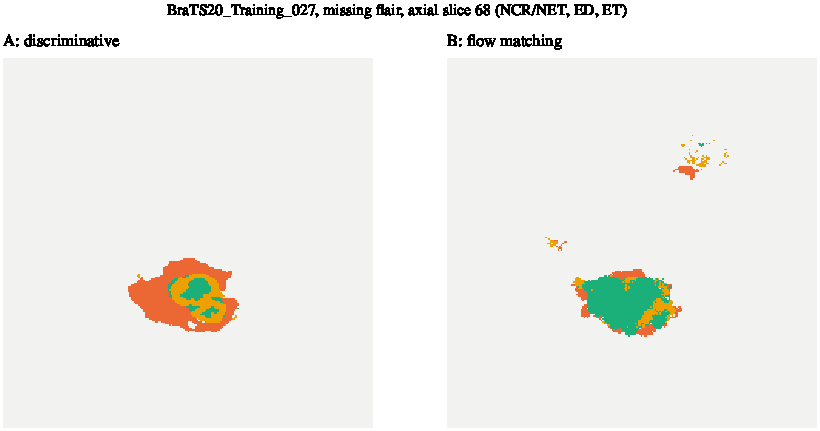
\includegraphics[width=\textwidth]{fig_qualitative.pdf}
\caption{One test patient with FLAIR withheld, axial slice through the tumour.
Model B over-segments the necrotic core and places false-positive islands far
from the tumour, while A follows the reference. Colours encode the three
foreground classes; the background is unfilled.}
\label{fig:qual}
\end{figure*}

\subsection{Diagnostic: what the collapse is not}
\label{sec:diag}

\paragraph{Check 1 --- not overfitting, not capacity.}
Fine-tuning on two training patients with balanced patch sampling, model A
reaches $0.941$ whole-tumour Dice on those patients with a median of $2$
connected components, while model B reaches $0.538$ with $5{,}569$ components.
On the full test split the train-to-test gap for B is only $0.058$, below the
pre-registered $0.10$ threshold. The task is fittable --- A demonstrates it ---
and B's deficit is present on the training patients themselves, so it is not a
generalisation problem.

\paragraph{Check 2 --- the model is conditioned, and the field is accurate on
average.}
Replacing the MRI conditioning with zeros or with a shuffled volume drives B's
Dice to $0.000$, and substituting another patient's MRI leaves it at $0.049$,
against $0.553$ with the real conditioning: B is genuinely using the MRI, well
beyond the pre-registered $0.05$ margin. On held-out patches the velocity field
has $R^2$ between $0.855$ and $0.966$ against the conditional target, and beats
a global-class-prior reference by factors of $1.8$ to $6$ in the low and middle
range of $t$. In $L_2$ terms the field is good.

\paragraph{Check 3 --- the error is not uniform, and it is not the background
distribution.}
The velocity error is not spread evenly over $t$: per-step RMS error rises by a
factor of $1.8$ from $0.231$ at $t \approx 0.06$ to $0.416$ at $t \approx 0.94$,
while the target variance is constant at $1.188$. Equivalently, $R^2$ falls from
$0.955$ to $0.855$ as $t \to 1$ --- exactly the direction predicted by the
$1/(1-t)$ factor of Eq.~(3). The error is also not uniform across classes: at
$t = 0.562$ the per-class MSE is $0.024$ for background against $0.164$,
$0.143$ and $0.191$ for NCR, ED and ET. Aggregate MSE therefore understates the
error in the region that decides the argmax by roughly six to eight times. Both
effects are visible in Figure~\ref{fig:mech}. We
tested the alternative explanation that B hallucinates because its background
distribution is mismatched: an augmentation variant that keeps the background
strictly zero raises B's test whole-tumour Dice by $0.007$ ($+0.022$ for A), so
the pre-registered $0.05$ threshold is not met.

\begin{figure*}[t]
\centering
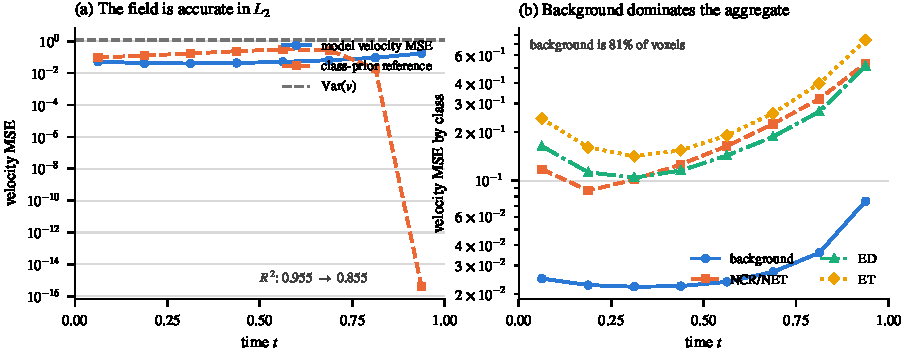
\includegraphics[width=\textwidth]{fig_mechanism.pdf}
\caption{(a) The learned velocity field is accurate in $L_2$ (note the log
scale): its MSE is far below the target variance and, in the low and middle
range of $t$, below a class-prior-only reference. The reference is meaningless
once $y_t$ nearly determines the answer, which is why that curve is not drawn
past $t\approx 0.8$. (b) The same error split by class: background sits two
orders of magnitude below the tumour classes, so the aggregate MSE in (a)
understates the error in the region that decides the argmax.}
\label{fig:mech}
\end{figure*}

\paragraph{Check 4 --- integration is not the bottleneck, and more steps are
worse.}
Sweeping Euler steps from $8$ to $128$ moves whole-tumour Dice monotonically
\emph{down} from $0.560$ to $0.483$; the pre-registered threshold for
``integration is not the bottleneck'' was a change below $0.02$, and we observe
$-0.034$ in the direction opposite to the one that a solver-error explanation
would require. A related measurement explains why: the median margin between the
largest and second-largest channel of the final continuous state is $0.984$ and
is invariant to step count ($0.983$ at $8$ steps and $0.984$ at $128$), brain
and non-brain alike ($0.978$ vs.\ $0.984$), and only $1.2\%$ of voxels have a
margin below $0.25$. Voxels that turn out to be wrong do carry a lower mean
margin ($0.52$ against $0.97$ for correct ones), so the margin is weakly
informative; but because almost no voxel is near a tie, the errors cannot be
dismissed as unresolved ambiguity. The endpoint is not a coin flip that better
integration would settle --- a more accurate solve of the same field simply
follows the trajectory further into the wrong answer. Figure~\ref{fig:sweep}
shows both effects.

\begin{figure*}[t]
\centering
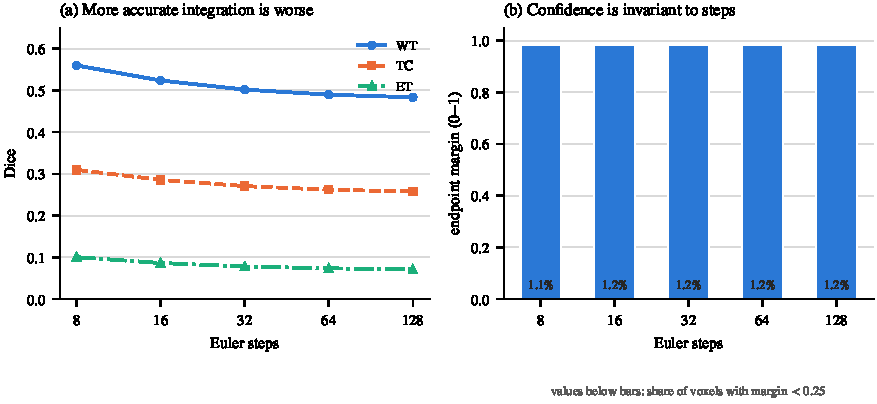
\includegraphics[width=\textwidth]{fig_sweep.pdf}
\caption{(a) Whole-tumour, tumour-core and enhancing-tumour Dice as a function
of the number of Euler steps: more accurate integration of the same field is
monotonically worse. (b) Mean endpoint decision margin, split by whether the
voxel is ultimately classified correctly: both curves are flat across step
counts. Wrong voxels are less confident than correct ones, so the margin carries
some information, but almost no voxel is near a tie.}
\label{fig:sweep}
\end{figure*}

\paragraph{Check 5 --- undertraining explains only a quarter of the gap.}
Training B for $40{,}000$ steps instead of $10{,}000$ raises test whole-tumour
Dice from $0.529$ to $0.599$, closing about a quarter of the gap to A, while A
reaches $0.803$ with a quarter of the updates. Model B's 40k-step curve is also
non-monotonic, with a collapse at $30{,}000$ steps.

\REMEDYSECTION

\begin{table}[t]
\centering
\caption{Binary whole-tumour task (three seeds, 20 test patients). Flow matching stays within $\sim$0.10 Dice here, unlike the four-class task in Table~\ref{tab:main}.}
\label{tab:binary}
\small
\setlength{\tabcolsep}{3pt}
\begin{tabular}{lcccc}
\toprule
Scenario & $A$ Dice & $B$ Dice & $A$ sec. & $B$ sec. \\
\midrule
C0 (all) & $0.878\pm0.005$ & $0.779\pm0.010$ & 0.39 & 5.93 \\
C1 (w/o T1ce) & $0.874\pm0.006$ & $0.780\pm0.014$ & 0.38 & 5.93 \\
C2 (T2+FLAIR) & $0.870\pm0.008$ & $0.776\pm0.015$ & 0.37 & 5.93 \\
\bottomrule
\end{tabular}
\end{table}


\section{Discussion}
\label{sec:discussion}

\paragraph{Cost.}
Sampling B costs $6.06$\,s per volume against $0.42$\,s for A, a factor of
$14.4$, and training costs $28.1$\,min against $11.1$\,min. Peak GPU memory is
$8.79$\,GB against $7.19$\,GB. Both models fit in a single consumer GPU, but the
generative model gives up $0.27$, $0.34$ and $0.37$ Dice on WT, TC and ET in
exchange for $14\times$ the inference latency and $2.5\times$ the training time.
In a clinical pipeline where a volume must be segmented per
patient per session, this is the dominant practical consideration.

\paragraph{Reproducibility.}
Re-running the same configuration with only the validation interval changed
reproduces the first $100$ updates bit-for-bit --- the data and noise generators
are deterministic functions of \texttt{(seed, step)} --- but from update $200$
a $10^{-7}$ floating-point difference is amplified to $1$--$6\%$ and saturates.
Two runs of the identical configuration therefore differ by about $\pm 0.02$
absolute Dice in validation score. A $40{,}000$-step run is consequently an
independent run rather than an extension of a $10{,}000$-step one, and part of
the spread across seeds reflects this chaos rather than a property of the model.
We report it because single-seed comparisons of generative segmentation models
at this scale are not reliable.

\paragraph{Limitations.}
The study uses $100$ patients from a single dataset and a single backbone; the
four-class conclusion may not transfer to larger models or to datasets whose
targets are less class-imbalanced. The endpoint-margin measurement covers three
patients and two missing patterns for one seed. We diagnose and test remedies
but do not claim a working fix unless the remedy results above support it. Our
HD95 follows the implementation in our codebase --- the $95$th percentile of the
pooled symmetric surface distances --- and is not the official BraTS scoring
implementation, so HD95 values should be read comparatively rather than as
absolute benchmark numbers. Finally, the bootstrap covers evaluation noise only;
training-seed variance is reported separately and the $36$ cells are not
corrected for multiple comparisons.

\section{Conclusion}

We set out to test whether flow matching is a useful generative alternative for
missing-modality 3D brain tumour segmentation, and found a sharp regime
boundary. On a binary whole-tumour target it is competitive at $15\times$ the
sampling cost; on a four-class target it fails by up to $0.37$ Dice, uniformly
across seeds, missing patterns and regions. A pre-registered diagnostic rules
out overfitting, capacity, integration error and background mismatch, and
locates the cause in the interaction between an unboundedly sensitive regression
target and a background-dominated $L_2$ objective. The practical implication for
practitioners is that a flow-matching objective should not be adopted for
near-deterministic, strongly class-imbalanced volumetric targets without
checking both mechanisms, and that inference cost should be counted as part of
the comparison.

\REMEDYCONCLUSION

\bibliographystyle{IEEEtran}
\bibliography{refs}

\end{document}
